\documentclass[../../../../main.tex]{subfiles}
\begin{document}
\section*{東大理科数学 2000年}

\subsection*{第1問}
[解]右のような座標をおく。対称性から、
楕円の中心 $D(0,a)$ とすると、$b>0$ として、
楕円の方程式は
\[ \frac{x^2}{b^2} + \frac{(y-a)^2}{a^2} = 1 \]
とかける。($\because$ BCと接し、軸がBCと平行) ここで、$X=\frac{x}{b}$、$Y=\frac{y}{a}$ なる変換を行うと、
楕円は
\[ P : X^2 + (Y-1)^2 = 1 \]
へ、直線AB: $x+y=1$ は、
\[ l : bX + aY = 1 \]
へ、各々うつる。以下、ABと楕円が接する条件をかんがえる。(対称性から、この時ACと楕円が接する条件も同じ)。
$l$ と $(0,1)$ のキョリが $1$ なら良いので、
\[ \frac{|a-1|}{\sqrt{a^2+b^2}} = 1 \]
両辺 $0$ 以上から2乗して、
\[ b^2 = 1 - 2a \cdots \text{①} \]

ここで、$a$ は $0 < a = \frac{1-b^2}{2} < 1 \iff 0 < 1-b^2 < 2 \implies b^2 < 1$ から
$0 < b < 1 \cdots \text{②}$ をみたす。

楕円の面積 $S$ は、
\[ S = \pi a b = \pi b \frac{1-b^2}{2} \quad (\because \text{①}) \]
である。$f(b) = b(1-b^2)$ とすると、$f'(b) = 1 - 3b^2$ から、下表をうる。

\begin{center}
\begin{tabular}{|c|c|c|c|c|c|}
\hline
$b$ & $0$ & $\cdots$ & $\frac{1}{\sqrt{3}}$ & $\cdots$ & $1$ \\
\hline
$f'$ & & $+$ & $0$ & $-$ & \\
\hline
$f$ & & $\nearrow$ & & $\searrow$ & \\
\hline
\end{tabular}
\end{center}

したがって、$S$ は $b = \frac{1}{\sqrt{3}}$ で最大値、$\frac{\pi}{2} \cdot \frac{1}{\sqrt{3}} \cdot \frac{2}{3} = \frac{\sqrt{3}}{9}\pi$ をとる。
\begin{flushright}
(終)
\end{flushright}

\begin{center}
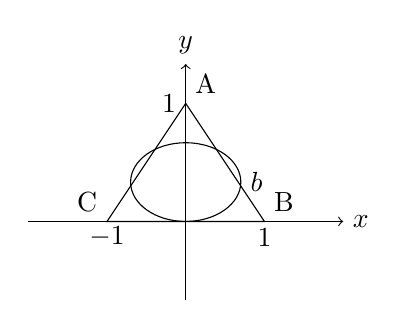
\begin{tikzpicture}
\draw[->] (-2,0) -- (2,0) node[right] {$x$};
\draw[->] (0,-1) -- (0,2) node[above] {$y$};
\draw (-1,0) -- (1,0) -- (0,1.5) -- cycle;
\node at (-1,-0.2) {$-1$};
\node at (1,-0.2) {$1$};
\node at (0,1.5) [left] {$1$};
\node at (-1,0) [above left] {C};
\node at (1,0) [above right] {B};
\node at (0,1.5) [above right] {A};
\draw (0,0.5) ellipse (0.7 and 0.5);
\node at (0.7,0.5) [right] {$b$};
\end{tikzpicture}
\end{center}

\subsection*{第2問}
[解] $OR \perp l$ から、
\[ \frac{w}{\alpha - \beta} \text{ は純虚数} \cdots \text{①} \]
さらに、Rは $l$ 上だから、$t \in \mathbb{R}$ として、
\[ (w - \beta) = t(\alpha - \beta) \]
\[ \therefore \frac{w-\beta}{\alpha-\beta} \in \mathbb{R} \cdots \text{②} \]
である。①、②から
\[ \begin{cases} \left( \frac{w}{\alpha-\beta} \right) + \overline{\left( \frac{w}{\alpha-\beta} \right)} = 0 \\ \left( \frac{w-\beta}{\alpha-\beta} \right) = \overline{\left( \frac{w-\beta}{\alpha-\beta} \right)} \end{cases} \]
\[ \begin{cases} w(\bar{\alpha}-\bar{\beta}) + \bar{w}(\alpha-\beta) = 0 \cdots \text{③} \\ (w-\beta)(\bar{\alpha}-\bar{\beta}) = (\bar{w}-\bar{\beta})(\alpha-\beta) \cdots \text{④} \end{cases} \]
まず、$w \neq 0$ だから、③から
\[ \bar{\alpha}-\bar{\beta} = -\frac{\bar{w}}{w}(\alpha-\beta) \]
だから、④に代入、セイリして、
\[ -(w-\beta)\frac{\bar{w}}{w}(\alpha-\beta) = (\bar{w}-\bar{\beta})(\alpha-\beta) \]
$\alpha \neq \beta, w \neq 0$ から、
\[ -(w-\beta)\bar{w} = w(\bar{w}-\bar{\beta}) \]
\[ 2|w|^2 - \bar{\beta}w - \beta\bar{w} = 0 \cdots \text{⑤} \]
同様にして、
\[ 2|w|^2 - \bar{\alpha}w - \alpha\bar{w} = 0 \cdots \text{⑥} \]
を得る。

$1^\circ$ 十分性
$w = \alpha\beta$ の時、⑤、⑥から、
\[ \begin{cases} 2|\alpha|^2|\beta|^2 - \alpha|\beta|^2 - \bar{\alpha}|\beta|^2 = 0 \\ 2|\alpha|^2|\beta|^2 - \beta|\alpha|^2 - \bar{\beta}|\alpha|^2 = 0 \end{cases} \]
$\alpha, \beta \neq 0$ だから、
\[ \left|\alpha - \frac{1}{2}\right|^2 = \frac{1}{4}, \quad \left|\beta - \frac{1}{2}\right|^2 = \frac{1}{4} \cdots \text{⑦} \]
となり、各辺 $0$ 以上だから
\[ \left|\alpha - \frac{1}{2}\right| = \frac{1}{2}, \quad \left|\beta - \frac{1}{2}\right| = \frac{1}{2} \cdots \text{⑧} \]
より、$P(\alpha), Q(\beta)$ は題意の円周上にある。

$2^\circ$ 必要性
⑧が成立するので、両辺2乗して⑦を得る。変形して、
\[ \begin{cases} \bar{\alpha} = \frac{\alpha}{2\alpha-1} \\ \bar{\beta} = \frac{\beta}{2\beta-1} \end{cases} \quad \left(\because \alpha, \beta \neq \frac{1}{2}\right) \cdots \text{⑨} \]
$A = \alpha - \beta$ とおく。$\alpha \neq \beta$ より $A \neq 0$ だから③より
\[ \bar{w} = -\frac{\bar{A}}{A}w \]
だから④に代入、セイリして、
\[ \left(-\frac{\bar{A}}{A}w - \bar{\beta}\right)A = (w - \beta)\bar{A} \]
\[ -\bar{A}w - \bar{\beta}A = \bar{A}w - \beta\bar{A} \]
\[ \beta\bar{A} - \bar{\beta}A = 2\bar{A}w \]
\[ w = \frac{\beta\bar{A} - \bar{\beta}A}{2\bar{A}} \]
\[ = \frac{\beta}{2} - \frac{1}{2} \left( \frac{\beta}{2\beta-1} \right) \frac{\alpha-\beta}{\frac{\alpha}{2\alpha-1} - \frac{\beta}{2\beta-1}} \quad (\because \text{⑨}) \]
\[ = \frac{\beta}{2} - \frac{1}{2} (2\alpha-1)\beta = \alpha\beta \]
を得る。
以上 $1^\circ$、$2^\circ$ から示された。
\begin{flushright}
$\blacksquare$
\end{flushright}

\begin{center}
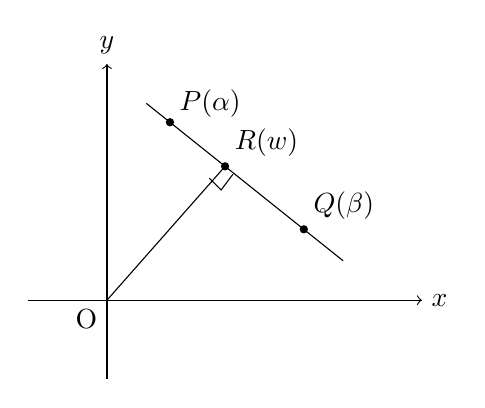
\begin{tikzpicture}
\draw[->] (-1,0) -- (4,0) node[right] {$x$};
\draw[->] (0,-1) -- (0,3) node[above] {$y$};
\node at (0,0) [below left] {O};
\draw (0.5,2.5) -- (3,0.5);
\node at (0.8,2.2) [above right] {$P(\alpha)$};
\fill (0.8,2.26) circle (1.5pt);
\node at (2.5,0.9) [above right] {$Q(\beta)$};
\fill (2.5,0.9) circle (1.5pt);
\draw (0,0) -- (1.5,1.7);
\node at (1.5,1.7) [above right] {$R(w)$};
\fill (1.5,1.7) circle (1.5pt);
\draw (1.3,1.55) -- (1.45,1.4) -- (1.6,1.6);
\end{tikzpicture}
\end{center}

\end{document}

\subsection*{第3問}
[解] (1) $f_n(kh) = q_k$ とおく。
(1) $q_0 = C \cdots \text{①}$
\[ \frac{q_{k+1}-q_k}{h} = (1-q_k)q_{k+1} \cdots \text{②} \]
$k \in \mathbb{Z}, k \ge 0$ の時、$q_k = 0$ と仮定する。この時②より、$ - \frac{q_k}{h} = 0 \iff q_{k+1} = 0$ となり、帰納的に $q_0 = 0$ が示される。しかしこれは $q_0 = C > 0$ に反し矛盾。したがって、任意の $0 \le k \le n, k \in \mathbb{Z}$ なる $k$ について、$q_k \neq 0$ である。②の両辺を $q_k q_{k+1} (\neq 0)$ でわると、
\[ \frac{p_k - p_{k+1}}{h} = p_k - 1 \quad \therefore p_{k+1} - 1 = (1-h)(p_k - 1) \]
だから、くり返し用いて $p_0 = \frac{1}{C}$ より、
\[ p_k = \frac{1-C}{C} (1-h)^k + 1 \]

(2) $kh = a$ に $h = \frac{a}{n}$ を代入して、$k=n$ だから、(1)より、
\[ f_n(a) = \frac{1}{\frac{1-C}{C} \left(1-\frac{a}{n}\right)^n + 1} = \frac{1}{\frac{1-C}{C} \left\{ \left(1-\frac{a}{n}\right)^{-\frac{n}{a}} \right\}^{-a} + 1} \xrightarrow{n \to \infty} \frac{1}{\frac{1-C}{C} e^{-a} + 1} \]
となり、
\[ g(a) = \frac{C}{C + (1-C)e^{-a}} \]

(3)
$C=2$ の時
$x > 0$ で $g(x) = \frac{2}{2-e^{-x}}$, $g'(x) = \frac{-2e^{-x}}{(2-e^{-x})^2} < 0$, $g''(x) = \frac{2e^{-x}(e^{-x}+2)}{(2-e^{-x})^3} > 0$
から、$g(x)$ は単調減少かつ下に凸。
又、$g(x) \xrightarrow{x \to +0} 2$, $g(x) \xrightarrow{x \to +\infty} 1$

$C=1$ の時
$g(x) = 1$

$C=\frac{1}{4}$ の時
$x > 0$ で $g(x) = \frac{1}{3e^{-x}+1}$, $g'(x) = \frac{3e^{-x}}{(3e^{-x}+1)^2} > 0$, $g''(x) = \frac{3e^{-x}(3e^{-x}-1)}{(3e^{-x}+1)^3}$
から右表を得る。又、$g(x) \xrightarrow{x \to +0} \frac{1}{4}$, $g(x) \xrightarrow{x \to +\infty} 1$

\begin{center}
\begin{tabular}{|c|c|c|c|c|}
\hline
$x$ & $0$ & $\cdots$ & $\log 3$ & $\cdots$ \\
\hline
$g'$ & & $+$ & $+$ & $+$ \\
\hline
$g''$ & & $+$ & $0$ & $-$ \\
\hline
$g$ & & $\nearrow$ & $\frac{1}{2}$ & $\nearrow$ \\
\hline
\end{tabular}
\end{center}

以上から、グラフは下図
\begin{center}
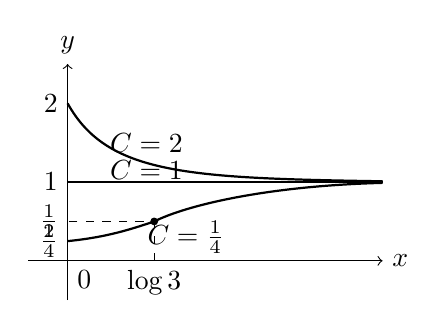
\begin{tikzpicture}
\draw[->] (-0.5,0) -- (4,0) node[right] {$x$};
\draw[->] (0,-0.5) -- (0,2.5) node[above] {$y$};
\draw[dashed] (0,1) -- (4,1);
\node at (0,1) [left] {$1$};
\node at (0,2) [left] {$2$};
\node at (0,0.25) [left] {$\frac{1}{4}$};
\node at (0,0) [below right] {$0$};
\draw[thick] (0,2) .. controls (0.5,1.1) and (1.5,1.05) .. (4,1.01);
\node at (1,1.5) {$C=2$};
\draw[thick] (0,1) -- (4,1);
\node at (1,1.15) {$C=1$};
\draw[thick] (0,0.25) .. controls (0.5,0.3) and (0.8,0.4) .. (1.1,0.5) .. controls (1.5,0.7) and (2.5,0.95) .. (4,0.99);
\node at (1.1,0.5) [circle,fill,inner sep=1pt] {};
\draw[dashed] (1.1,0) -- (1.1,0.5) -- (0,0.5);
\node at (1.1,0) [below] {$\log 3$};
\node at (0,0.5) [left] {$\frac{1}{2}$};
\node at (1.5,0.3) {$C=\frac{1}{4}$};
\end{tikzpicture}
\end{center}

\subsection*{第4問}
[解] 以下 $y = \cos t, y = 1-vt$ とおく。
P と線分 QR がぶつかるのは、$k \in \mathbb{Z}$ として、
\[ \begin{cases} 2k\pi + \frac{\pi}{3} \le t \le 2k\pi + \frac{2}{3}\pi \\ \cos t = 1 - vt \end{cases} \cdots \text{①} \]
をみたす時である。

(1) $0 \le t \le 2\pi$ で①をみたす $t$ がない時、まず $k=0$ として良い。
$y = \cos t$, $y = 1 - vt$ が共有点を持たない条件をもとめれば良い。
$t = \alpha$ における $y = \cos t$ の接線は $(y') = -\sin t$ から
\[ y = -\sin\alpha(t - \alpha) + \cos\alpha \]
これが $(0,1)$ を通る時、
\[ \alpha\sin\alpha + \cos\alpha = 1 \cdots \text{②} \]
この左辺 $f(\alpha)$ とすると
\[ f'(\alpha) = \alpha\cos\alpha \]
だから、下表をうる。

\begin{center}
\begin{tabular}{|c|c|c|c|c|c|}
\hline
$\alpha$ & $0$ & $\cdots$ & $\frac{\pi}{2}$ & $\cdots$ & $\frac{2}{3}\pi$ \\
\hline
$f'$ & & $+$ & $0$ & $-$ & \\
\hline
$f$ & $1$ & $\nearrow$ & $\frac{\pi}{2}$ & $\searrow$ & $\frac{\sqrt{3}}{3}\pi - \frac{1}{2}$ \\
\hline
\end{tabular}
\end{center}

$\left( \frac{\sqrt{3}}{3}\pi - \frac{1}{2} > 1 \iff \pi^2 > \frac{27}{4} \text{ で、}\pi=3.14\dots \text{ からこれは成立} \right)$
したがって、$\left[\frac{\pi}{3}, \frac{2}{3}\pi\right]$ では $f(\alpha) > 1$ だから、②をみたす $\alpha$ はないので、図から求める条件は、
\[ -\frac{\frac{3}{2}}{\frac{2}{3}\pi} > -v, \quad -v > -\frac{\frac{1}{2}}{\frac{1}{3}\pi} \quad \therefore v < \frac{3}{2\pi}, v > \frac{9}{4\pi} \]

(2) $y = \cos t$ と $y = 1 - vt$ が、①の区間内でただ1度交わる条件をしらべる。
ここで、$f(\alpha)$ について、$\left[2k\pi, (2k+\frac{2}{3})\pi\right]$ での増減表は下図

\begin{center}
\begin{tabular}{|c|c|c|c|c|c|}
\hline
$\alpha$ & $2k\pi$ & $\cdots$ & $(2k+\frac{1}{2})\pi$ & $\cdots$ & $(2k+\frac{2}{3})\pi$ \\
\hline
$f'$ & & $+$ & $0$ & $-$ & \\
\hline
$f$ & $1$ & $\nearrow$ & $(2k+\frac{1}{2})\pi$ & $\searrow$ & $\sqrt{3}(k+\frac{1}{3})\pi - \frac{1}{2}$ \\
\hline
\end{tabular}
\end{center}

$\left( \sqrt{3}(k+\frac{1}{3})\pi - \frac{1}{2} > \frac{\sqrt{3}}{3}\pi - \frac{1}{2} > 1 \right)$
したがって、$\left[(2k+\frac{1}{3})\pi, (2k+\frac{2}{3})\pi\right]$ では $1 < f(\alpha)$ で、①をみたす $\alpha$ は存在しないので、上のグラフから、
区間 $[2k\pi, 2(k+1)\pi]$ で1回 P と QR がぶつかる条件は
\[ \frac{-\frac{3}{2}}{(2k+\frac{2}{3})\pi} \le -v \le \frac{-\frac{1}{2}}{(2k+\frac{1}{3})\pi} \]
\[ \frac{1}{2(2k+\frac{1}{3})\pi} \le v \le \frac{3}{2(2k+\frac{2}{3})\pi} \cdots \text{②} \]
である。したがって、②をみたす $k \in \mathbb{Z}_{\ge 0}$ がただ1つある $v$ の範囲を求めれば良い。②を図示すると右上図
$\left( \frac{1}{2(2k+1/3)\pi} \le \frac{3}{2(2k+4+2/3)\pi} \iff \frac{11}{12} \le k \text{ 及び②の両辺が } k \text{ の単調減少関数であることから } 2 \le k \text{ の時、②をみたす } k \text{ がただ1つあることはありえない。} \right)$
したがって、求める範囲は、
\[ \frac{9}{28\pi} < v \le \frac{9}{16\pi}, \quad \frac{3}{2\pi} < v \le \frac{9}{4\pi} \]
である。

\begin{center}
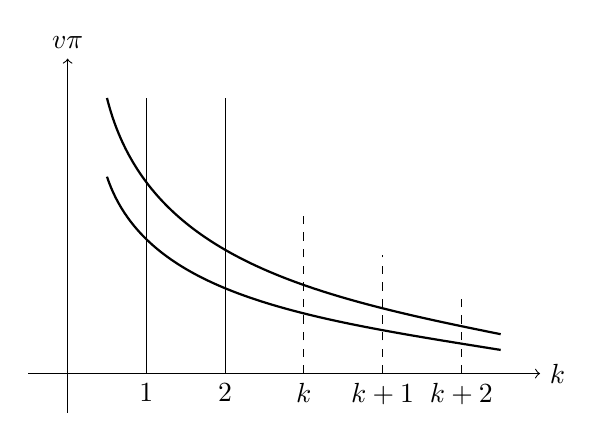
\begin{tikzpicture}
\draw[->] (-0.5,0) -- (6,0) node[right] {$k$};
\draw[->] (0,-0.5) -- (0,4) node[above] {$v\pi$};
\draw (1,0) -- (1,3.5);
\draw (2,0) -- (2,3.5);
\node at (1,0) [below] {$1$};
\node at (2,0) [below] {$2$};
\node at (3,0) [below] {$k$};
\node at (4,0) [below] {$k+1$};
\node at (5,0) [below] {$k+2$};
\draw[dashed] (3,0) -- (3,2);
\draw[dashed] (4,0) -- (4,1.5);
\draw[dashed] (5,0) -- (5,1);
\draw[thick] (0.5,3.5) .. controls (1,1.5) and (3,1) .. (5.5,0.5);
\draw[thick] (0.5,2.5) .. controls (1,1) and (3,0.7) .. (5.5,0.3);
\end{tikzpicture}
\end{center}

\subsection*{第5問}
[解] $0 \sim 9$ のセイスウを、足して $9$ になる2つずつで組をつくると、以下のように5組できる。
(0,9) (1,8) (2,7) (3,6) (4,5) $\cdots$ ①
A \quad B \quad C \quad D \quad E

(1) S のうち4ケタのものは、①の中から4つの組をえらび、4位に0がこないよう注意しながら、
4組のうちいずれか一方を配分したものである。
4位に0が来てもいい時の場合の数は、
\[ {}_5C_4 \times 2^4 \times 4! = 1920 \text{コ} \cdots \text{②} \]
である。このうち、4位が0であるのは、
\[ {}_4C_3 \times 2^3 \times 3! = 192 \text{コ} \cdots \text{③} \]
だから、求める数は $1920 - 192 = 1728 \text{コ}$ である。

(2) (1)と同様に数えると、
1ケタのもの $\cdots$ 9コ
2ケタのもの $\cdots$ 72コ
3ケタのもの $\cdots$ 432コ
合わせて 513コ
だから、Sの要素を小さいものから並べた数列 $\{a_n\}$ において、4ケタの数は、$a_{514} \sim a_{2241}$ で
ある。つまり、$S_{2000}$ は 4ケタの数。Sの4ケタの数のうち、4ケタ目が $k$ ($1 \le k \le 9$) であるものは
③と同様に数えて 192コ あるから、
\[ 513 + (k-1) \cdot 192 < 2000 < 513 + k \cdot 192 \]
をみたす $k \in \mathbb{N}$ は、$k=8$ であることとあわせて、$S_{2000}$ の4位は 8 である。さらに、$S_{2000}$ は 4位
が 8 であるもののうち、小さい方から数えて、
\[ 2000 - 1857 = 143 \text{ 番目} \]
である。
次に、3位について、4位が8の時は①のうち残り A, C, D, E から 3つをえらぶことより、
3位が $l$ ($l = 0,2,3,4,5,7,9$) である場合の数は、
\[ {}_3P_2 \times 2^2 = 24 \text{コ} \]
である。よって、
\[ 24(m-1) < 143 \le 24m \]
をみたす $m \in \mathbb{N}$ は $m = 6$ だから、6番目の数字である $l=6$ である。さらに $S_{2000}$ は、$8 6 \square \square$ の形でかける
S の要素のうち、一番大きい方から
\[ 144 - 143 + 1 = 2 \text{ 番目} \]
で、順に書き下すと、
8697, 8695
だから、$S_{2000} = 8695$
\begin{flushright}
(終)
\end{flushright}

\subsection*{第6問}
% Blank page in original
\end{document}
